\documentclass{report}
\usepackage[margin=0.9in]{geometry}
\usepackage{minted,graphicx}
\setminted{linenos, frame=single}
\usemintedstyle{xcode}
\usepackage{titlesec}
\titleformat{\chapter}[display]
{\normalfont%
    \huge% %change this size to your needs for the first line
    \bfseries}{\chaptertitlename\ \thechapter}{18pt}{%
    \huge %change this size to your needs for the second line
    }


\usepackage{hyperref}
\begin{document}
\begin{titlepage}
    \title{ECPE-174 Final Project: Simon Says \\ \large{University of the Pacific: School of Engineering and Computer Science}}
    \author{Mari Anderson and Felix Pitts}
    \maketitle
\end{titlepage}
\tableofcontents
\newpage
\chapter{Project Overview and Objectives}
\section{Overview}
The project involves creating a "Simon Says" memory game on a programmable board. This game challenges players to mimic a sequence of LEDs by toggling keys in the correct order. As rounds progress, the sequence becomes longer and more difficult, testing the player's memory and reaction time. The game integrates a visual (LCD Display) interface to enhance user engagement.
\section{Objectives}
\begin{enumerate}
    \item Develop a Memory game
    \begin{itemize}
        \item Implement a sequence-based gameplay mechanism where LEDs display an increasing pattern.
        \item Require players to input the pattern via keys to progress through rounds.
    \end{itemize}
    \item  Increase Challenge Progressively
    \begin{itemize}
        \item Add a new LED to the sequence in each round, making it more challenging for players to recall and replicate.
    \end{itemize}
    \item Display Real Time Information
    \begin{itemize}
        \item Use a LCD Display to provide critical feedback
        \begin{itemize}
        \item[$\circ$] Current round number
        \item[$\circ$] High score across multiple games 
        \end{itemize}
    \end{itemize}
    \item Support High Score Tracking
    \begin{itemize}
        \item Ensure that high scores persist across game sessions, motivating players to achieve better results over time.
    \end{itemize}
    \item Test for Scalability
    \begin{itemize}
        \item Design the game to support up to 100 rounds for testing purposes, even if impractical for real-time play.
    \end{itemize}
\end{enumerate}

\chapter{Design Process}
\section{System Design}
Our system design began with the following diagram
\begin{figure}[H]
    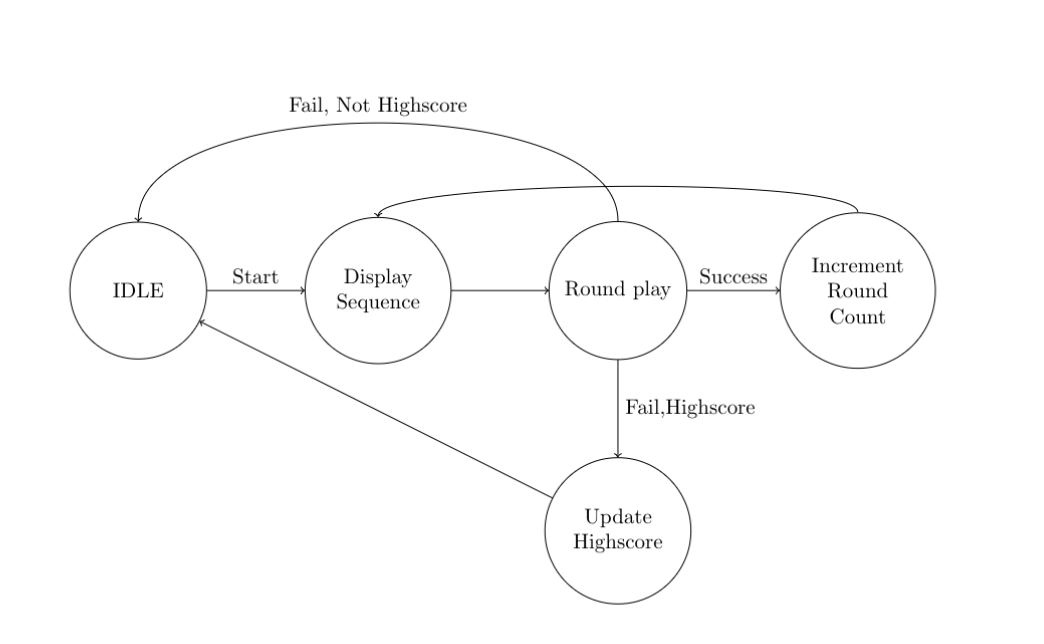
\includegraphics[width=\textwidth]{images/image4.png}
    \caption{Diagram for the States of the Game}
\end{figure}
The diagram in Figure 1 was the basis for how the FSM that we use to run the game was designed. The Transitions that occur are the following
\begin{itemize}
    \item \textbf{IDLE $\rightarrow$ Display Sequence:} When any button is pressed on the board
    \item \textbf{Display Sequence $\rightarrow$ Round Play:} Once the sequence is done displaying, the board accepts user input
    \item \textbf{Round Play $\rightarrow$ Increment Round Count:} If the user succeeds in replicating the input sequence displayed by the board, the round count increases
    \item \textbf{Increment Round Count $\rightarrow$ Display Sequence:} Once the round count has increased by one, the sequence is then displayed again but with 1 more term than the sequence displayed in the previous round
    \item \textbf{Round Play $\rightarrow$ IDLE:} When a player either makes a mistake or takes too long to input the sequence but does not get the high score, the game returns back to an IDLE state
    \item \textbf{Round Play $\rightarrow$ Update Highscore:} If the highscore was obtained, update the highscore at the end of the round before going back to IDLE
    \item \textbf{Update Highscore $\rightarrow$ IDLE:} After the highscore has been updated return to IDLE.
\end{itemize}
While the final FSM does not follow this exactly, it created a structure that made writing the System Verilog code much easier. Some of the differences between the diagram in Figure 1 and the final result would be that even if the highscore is not obtained, the FSM goes into a "Round Lost" state, and checks for the highscore in that state, instead of going to a state if the highscore is obtained. The implementation is explored further in \hyperlink{round_lost}{Section 2.3} \newline
\newline
Another difference is that the round incrementing occurs in the Round Play State when the number of correct inputs matches the number of terms being displayed in the sequence.
\begin{figure}[H]
\begin{minted}{sv}
if (subRound >= currRound) begin
    subRound = 8'd0;
    currRound = currRound + 8'd1;
    next_state = DISPLAY_SEQUENCE;
end else begin
    next_state = ROUND_PLAY;
end
\end{minted}
\caption{Code Snippet from \texttt{ROUND\char`_PLAY} state that handles Incrementing the Round Count}
\end{figure}
These differences in the final design did not hinder the functionality of the game, and by keeping the number fo states down to 4, we can represent our states with 2 bit values, and have no unused states.   
\newpage
\section{Hardware Design}
For hardware design we broke the design down into the following parts.
\begin{enumerate}
    \item \textbf{LED Display:}
    \begin{itemize}
        \item LEDs are used to visually display the game sequence that players need to replicate. Each LED corresponds to a switch for user input.
    \end{itemize}
    \item \textbf{Key Inputs:}
    \begin{itemize}
        \item Keys serve as the primary user interface for entering the sequence. They are debounced to ensure accurate input capture. This replaced the initial concept design of using switches.
    \end{itemize}
    \item \textbf{Seven Segment Display}
    \begin{itemize}
        \item Displays real-time game information, including the current round number and high score. This replaced the initially planned LCD display to ensure reliability and ease of integration.
    \end{itemize}
    \item \textbf{Programmable board}
    \begin{itemize}
        \item Serves as the central processing unit, executing the state machine logic and controlling all hardware components.
    \end{itemize}
    \item \textbf{External Clock}
    \begin{itemize}
        \item A clock divider generates game-specific timing signals, ensuring synchronized operation of game states and LED sequences.
    \end{itemize}
    \item \textbf{Finite State Machine (FSM):}
	\begin{itemize}
		\item Governs the games behavior, ensuring logical transitions between the states of the game.
		\item Takes care of the error handling, ensuring that when the incorrect button is pressed the game goes a failure state before going back to IDLE
	\end{itemize}
    \item \textbf{Random Sequence Generator:}
		\begin{itemize}
		\item Creates unique sequences for each round, ensuring variability and challenge for the players 
		\end{itemize}
\end{enumerate}
\section{Finite State Machine Design}\label{FSM_DESIGN}
For the final FSM that we used for the board hardware there were 4 states. \texttt{IDLE},  \texttt{DISPLAY\char`_SEQUENCE}, \texttt{ROUND\char`_PLAY}, and \texttt{ROUND\char`_LOST}. The roles that the states filled was the following
\begin{enumerate}
    \item \texttt{IDLE}
    \begin{itemize}
        \item Waits for any user input on the 4 buttons on the FPGA board to start the game
        \item Keeps the game at an IDLE state when there is no Input
        \item Sets the start signal to 0 so that the system can generate a random sequence when the game is not being played
    \end{itemize}
    \begin{figure}[H]
        \begin{minted}{sv}
IDLE:
begin
    currRound <= 8'd0;
    play_led <= 1'b0;
    start <= 1'b0;
    if (synced_keys != 4'b0000) begin
        next_state <= DISPLAY_SEQUENCE;
        currRound <= 8'd1;
    end else begin
        next_state <= IDLE;
    end
end
        \end{minted}
        \caption{IDLE State System Verilog Code}
    \end{figure}
    \item \texttt{DISPLAY\char`_SEQUENCE}
    \begin{itemize}
        \item Starts the display at the first element of the sequence when coming from IDLE or ROUND PLAY 
        \item Lights up one of the LEDS depending on what the value of the sequence at that point is
        \item When done displaying the sequence transitions into ROUND PLAY
    \end{itemize}
    \begin{figure}[H]
        \begin{minted}{sv}
DISPLAY_SEQUENCE:
begin
    start <= 1'b1;
    play_led <= 1'b0;
    if (prev_state == IDLE || prev_state == ROUND_PLAY) begin
        subRound <= 8'd0;
    end else begin
        subRound <= subRound;
    end
    if (subRound >= currRound )begin
        subRound <= 8'd0;
        next_state <= ROUND_PLAY;
    end else begin
        case (genned_sequence[subRound])
            2'b00: key_leds <= 4'b0001; //LEDG0
            2'b01: key_leds <= 4'b0010; //LEDG2
            2'b10: key_leds <= 4'b0100; //LEDG4
            2'b11: key_leds <= 4'b1000; //LEDG6
            default: key_leds <= 4'b0000;
        endcase
        seq_disp_count <= seq_disp_count + 8'd1;
        if (seq_disp_count == 5'b11111) begin
            subRound <= subRound + 8'd1;
            seq_disp_count <= 5'd0;
        end else begin
            subRound <= subRound;
        end
        next_state <= DISPLAY_SEQUENCE;
    end
end
        \end{minted}
        \caption{\texttt{DISPLAY\char`_SEQUENCE} State System Verilog Code}
    \end{figure}
    \item \texttt{ROUND\char`_PLAY}
    \begin{itemize}
        \item Starts taking user input for the start of the sequence when the round begins
        \item Resets the round timer to 0 at the start of the round and then counts up the longer the round has been progressing
        \item If the input is wrong or the timer ran out, transitions to \texttt{ROUND\char`_LOST}
        \item Goes to \texttt{DISPLAY\char`_SEQUENCE} when the round is successfully completed
    \end{itemize}
    \begin{figure}[H]
    \small{\inputminted{sv}{ROUND_PLAY.sv}}
    \caption{\texttt{ROUND\char`_PLAY State System Verilog Code}}
    \end{figure}
    \item \hypertarget{round_lost}{\texttt{ROUND\char`_LOST}}
    \begin{itemize}
        \item Checks if the Highscore was beaten, if so updates the value stored.
        \item Prepares the system to return back to \texttt{IDLE}
    \end{itemize}
    \begin{figure}[H]
        \begin{minted}{sv}
ROUND_LOST:
begin
    if (currRound > high_score) begin
        high_score <= currRound;
    end else begin
        high_score <= high_score;
    end
    key_leds <= 4'b0000;
    play_led <= 1'b0;
    next_state <= IDLE;
    currRound <= 8'd0;
    round_timer <= 12'd0;   
end
        \end{minted}
    \end{figure}
\end{enumerate}
Intel Quartus generated a state diagram for the FSM we created but due to the code being in an \mintinline{sv}|always @()| block instead of an \mintinline{sv}|always_comb| block the FSM Diagram generated is incorrect from what actually happens with the FSM.
\begin{figure}[H]
    \begin{center}
    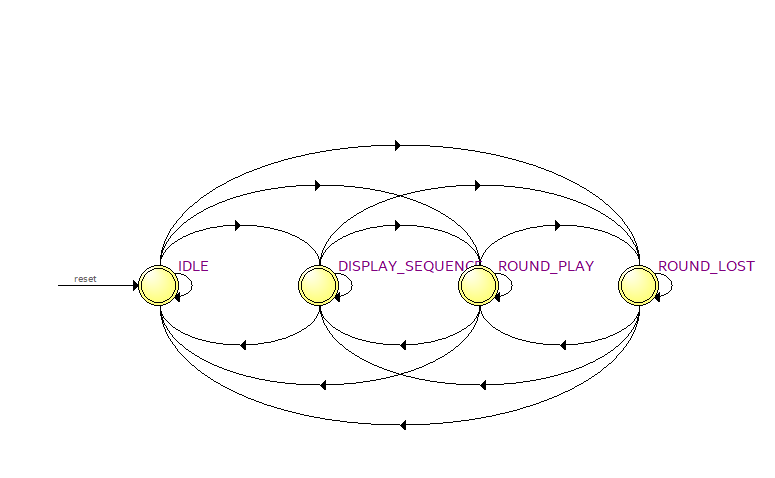
\includegraphics[scale = 0.9]{images/image2.png}
    \end{center}
    \caption{FSM Diagram Generated From Quartus}
\end{figure}
The reason an \mintinline{sv}|always @()| block was used was that we had to use sequential logic for the \texttt{ROUND\char`_PLAY} state to get it to function as intended. We did try to use an \mintinline{sv}|always_comb| block, however I could not get it to compile despite many hours of debugging. The Full FSM Code, which was also the Top Level Module can be found in the \hyperlink{fsm_code}{Appendix}


\newpage
\section{Random Sequence Generation}
\subsection{Seed Generation}
For the random number generation we need a way to generate the input value for the random number generator to be able to work. The way we do this is by counting the number of clock cycles that have occurred on the hardware. In the case of the FPGA used for the game, the Terasic DE2-115, that clock is 50MHz, so it is fast enough to where no human could hope to manipulate the random number generation with any reliable consistency without the use of external hardware directly connected to the system.
\begin{figure}[H]
    \inputminted{sv}{../seedgenerator.sv}
    \caption{Seed Generation System Verilog Code}
\end{figure} 
Once the seed has been generated, we can then go create a pseudo random number.
\subsection{Random Number Generation}
For the Random Number Generation we used an XOR-Shift algorithm, as it was very straightforward to translate from C into System Verilog
\begin{figure}[H]
    \inputminted{C}{../xorshift.c}
    \caption{C Code for XOR-Shift RNG Generation (From \href{https://en.wikipedia.org/wiki/Xorshift}{Wikipedia})}
\end{figure} 
How the algorithm in Figure 1 works is that it takes an unsigned 32-bit integer as an input, then performs XOR operations with the initial value, and that value bit shifted by an arbitrary amount. For example the code in Figure 1 does the following steps
\begin{itemize}
    \item set x to the input a
    \item set x to x XOR (x shifted left 13 bits)
    \item set x  to x XOR (x shifted right 17 bits)
    \item set x to x XOR (x shifted left 5 bits)
    \item return x
\end{itemize}
Because this algorithm uses binary bit operations translating this to System Verilog is very straightforward.
\begin{figure}[H]
    \inputminted{sv}{../xorshift.sv}
    \caption{XOR-Shift implementation in System Verilog}
\end{figure}
The main difference between Figure 1 and Figure 2 is that for Figure 2 we have to declare dedicated intermediate values due to the mechanics of System Verilog. With our modules for seed and RNG generation we can put them together to form a module that takes handles the random number generation.
\begin{figure}[H]
    \inputminted{sv}{../rng_generation.sv}
    \caption{Random Number Generation Module System Verilog Code}
\end{figure}
\subsection{Sequence Generation}
\begin{figure}[H]
    \inputminted{sv}{../sequence_generation.sv}
    \caption{Sequence Generation System Verilog Code}
\end{figure}
Here the code in Figure 2.11 takes in the RNG value generated in Figure 2.10, and uses that to generate a sequence of 100 values between 0 and 3. The sequence moves throughout the array until the \verb|start| signal is high, which is triggered when the round starts so that the sequence does not change on the user while they are playing the game.
\chapter{Testing Procedure}

\section{Seedgenerator Testbench}
\begin{figure}[H]
    \inputminted{sv}{../seedgenerator_testbench.sv}
    \caption{Seed Generator Testbench System Verilog Code}
\end{figure}
The file \verb|seedgenerator_testbench.sv| is designed to test the functionality of the seed generator module. Here's a breakdown of its purpose and components:
\begin{enumerate}
    \item \textbf{Clock Signal Generation:}
    \begin{itemize}
        \item A clock signal (clk) is toggled every 10 time units using an always block (\texttt{\char`#}10 clk = ~clk;). This simulates a regular clock input to the seedgenerator module.
    \end{itemize}
    \item \textbf{Module Under Test (MUT):}
    \begin{itemize}
        \item The seedgenerator module is instantiated with two ports:
        \begin{itemize}
            \item clk: The clock signal generated in the testbench.
            \item seed (mapped to a): An output signal from the seedgenerator module, expected to provide a generated seed value.
        \end{itemize}
    \end{itemize}
    \item \textbf{Simulation Monitoring}
    \begin{itemize}
        \item The \verb|$monitor| task is used to continuously display the values of the clock (clk) and the generated seed (a) during simulation. This provides real-time insight into how the module responds to the clock input.
    \end{itemize}
    \item \textbf{Purpose}
    \begin{itemize}
        \item The testbench evaluates how the seedgenerator module generates or updates the seed (a) in response to the clock signal. By observing the outputs, you can verify whether the module behaves as expected.
    \end{itemize}
\end{enumerate}
This testbench is straightforward, focusing on ensuring that the clock signal and module outputs function correctly in a basic simulation environment.

\section{XORshift Testbench}
\begin{figure}[H]
    \inputminted{sv}{../xorshift_testbench.sv}
    \caption{System Verilog Code for the xorshift Test Bench}
\end{figure}
From there to reduce file size to make computing information on this data easier the output file is ran throughout the following python script:
\begin{figure}[H]
    \inputminted{python}{../output_fix.py}
    \caption{Python Script to Reduce the File Size of the Testbench Output}
\end{figure}
Questa adds a lot of whitespace into the output file, which adds no extra information but increases the file size dramatically, which is why we need the script in Figure 4. Running our output file through the script changed the file size from 682.7 MB to 105.0 MB, so a very large reduction in file size. Then to validate that the output is a uniform distribution the fixed output file is run through the following Python code in a Jupyter Notebook.
\begin{figure}[H]
    \inputminted{python}{../meow.py}
\end{figure}
Using that code after simulating around 52.5 million generated values creates the following plot:
\begin{figure}[H]
    \begin{center}
        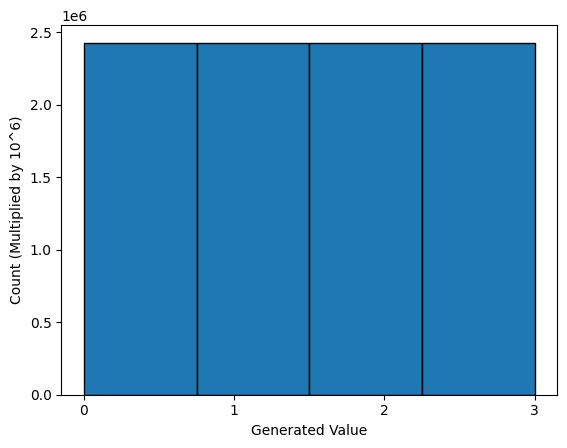
\includegraphics[scale=0.5]{images/rng_plot.png}
    \end{center}
\end{figure}
From this plot we can see that we get a distribution that is uniform. Looking at the number of times each value (0,1,2,3) occurred we can see that the differences in how many times each number is generated is very small
\begin{figure}[H]
    \begin{Verbatim}[frame=single]
0: 13128782, 1: 13128785, 2: 13128783, 3: 13128783
    \end{Verbatim}
    \caption{Number of Times each Generated Value Occurred in the Simulation}
\end{figure}
 \newpage
\section{Sequence Generation Testbench}
\begin{figure}[h]
    \inputminted{sv}{../sequence_testbench.sv}
    \caption{Sequence Generator Testbench System Verilog Code}
\end{figure}

The testbench for the \verb|sequence generation| module (\verb|sequence_generation|) is designed to verify that the sequence of game states is being generated and stored correctly in the \verb|game_sequence| array. The module under test, \verb|sequence_generation|, is instantiated with a clock (clk) and the output \verb|sequence array| (\verb|game_sequence|). The sequence output is stored and logged in a CSV file for analysis. The module generates 10, 100 value sequences and by storing them in a CSV file we were able to use a spreadsheet software to validate that the sequences were 100 values long, and that the wrap around worked. In summary, our testbench effectively verified the core functionality of the sequence generation module. We chose a straightforward approach of logging the output to a file and ensuring that the sequence generation was correct across multiple rounds. By focusing on key test cases, such as full sequence generation and boundary conditions, we ensured the robustness of the system while keeping the testbench design simple and efficient.

\newpage
\section{Top Module Testbench}
The \verb|Game_tb| testbench was designed to thoroughly test the Game module, which simulates a "Simon Says" game where players interact with the system using keys and observe outputs on LEDs and displays. The testbench was structured to cover several different scenarios of key presses to validate the correct operation of the game.
\subsection{Testbench Design Approach}
\begin{enumerate}
    \item \textbf{Clock Generation}
    \begin{itemize}
        \item A clock signal is generated with a period of 10 ns (100 MHz) using the forever construct. This ensures the system operates at a consistent frequency for all test cases.
    \end{itemize}
    \item \textbf{Stimulus}
    \begin{itemize}
        \item A variety of test cases were written to simulate key presses and observe the corresponding outputs. This includes:
        \begin{itemize}
            \item \textbf{No Key Pressed:} The system is initialized with no keys pressed (keys = 4'b0000), testing the default behavior of the game.
            \item \textbf{Single Key Pressed:} A test case where only one key is pressed (keys = 4'b0001), verifying that individual key presses are correctly recognized.
            \item \textbf{Multiple Keys Pressed:} Two keys are pressed (keys = 4'b1010), testing the system's ability to handle multiple inputs.
            \item \textbf{All Keys Pressed:} A case where all keys are pressed (keys = 4'b1111), ensuring the system can process all inputs simultaneously.
        \end{itemize}
    \end{itemize}
    \item \textbf{Coverage}
    \begin{itemize}
        \item \textbf{Outputs Monitoring:} For each test, the testbench monitors both the LED outputs (\verb|play_led| and \verb|key_leds|) and the seven-segment display outputs (display0 to display7). This ensures the visual feedback from the game is correct based on the key inputs.
        \item \textbf{Randomization: } The testbench does not utilize randomization as the main goal is to cover specific, deterministic key press cases. This approach is appropriate as it allows for a predictable evaluation of the system's response to particular input scenarios.
        \item \textbf{Reset and Stability:} The design tests multiple key press scenarios in sequence, ensuring the system's stability and correctness after each change in input. The system's reaction to different input combinations (none, one, or many keys) is observed, covering normal operating conditions.
    \end{itemize}
    \item \textbf{Additional Considerations}
    \begin{itemize}
        \item The testbench checks the functionality of both LEDs and displays to ensure all visual indicators work as expected for a range of key inputs.
        \item The use of the \verb|#|10 delay between key changes ensures that the system has time to process the inputs and update the outputs, simulating a real-time game environment.
    \end{itemize}
\end{enumerate}
By writing tests that check individual and combined key presses, the testbench provides a comprehensive assessment of the Game module, verifying its ability to respond to expected input patterns and display the correct outputs.
\chapter{Results}
We were unable to include memory into our project however we were still able to save the current high score of the game. We were also unsuccessful in getting the LCD screen to display any results or feedback as this was a challenging aspect of the final project. We instead resulted in using the Seven Segment display which was much easier as we were running out of time. The game was successful in working however in terms of randomizing the pattern of the game we usually got a consistent pattern due to the RNG only randomizing 4 values.
\begin{figure}[H]
    \begin{center}
        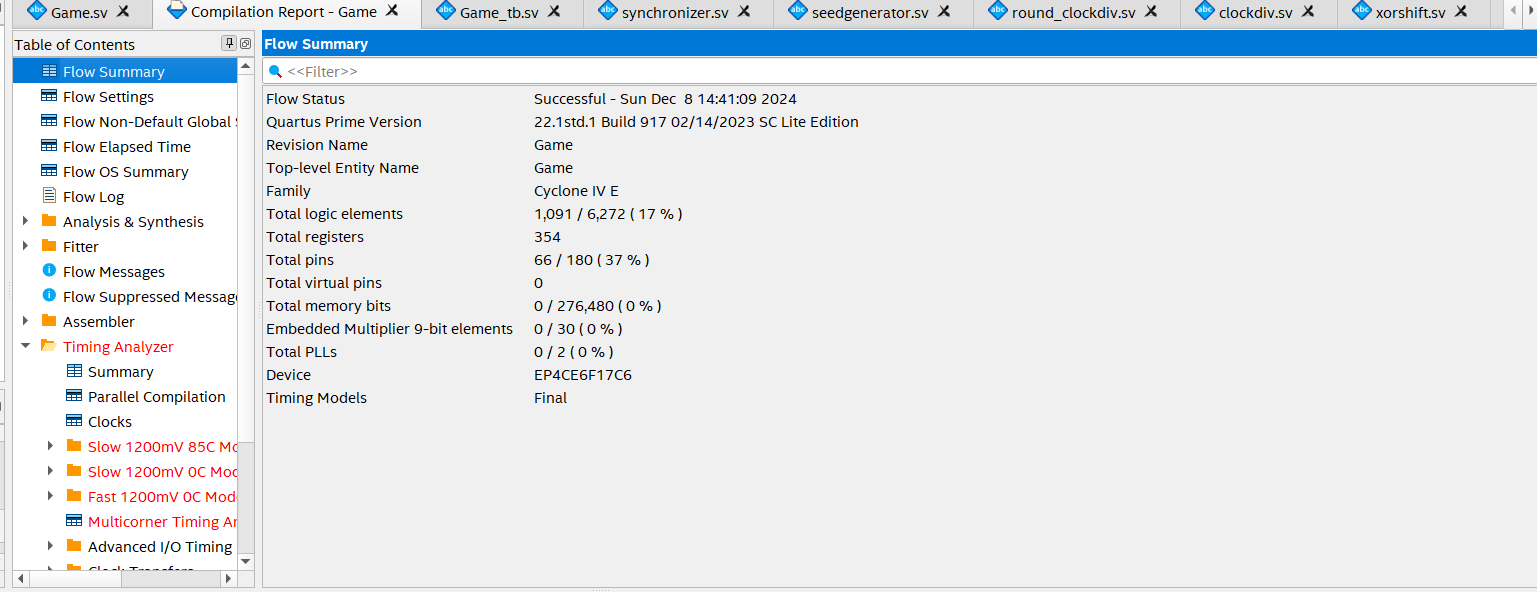
\includegraphics[width=0.75\textwidth]{images/image3.png}
    \end{center}
    \caption{Intel Quartus Compilation Report}
\end{figure}
\begin{figure}[H]
    \begin{center}
        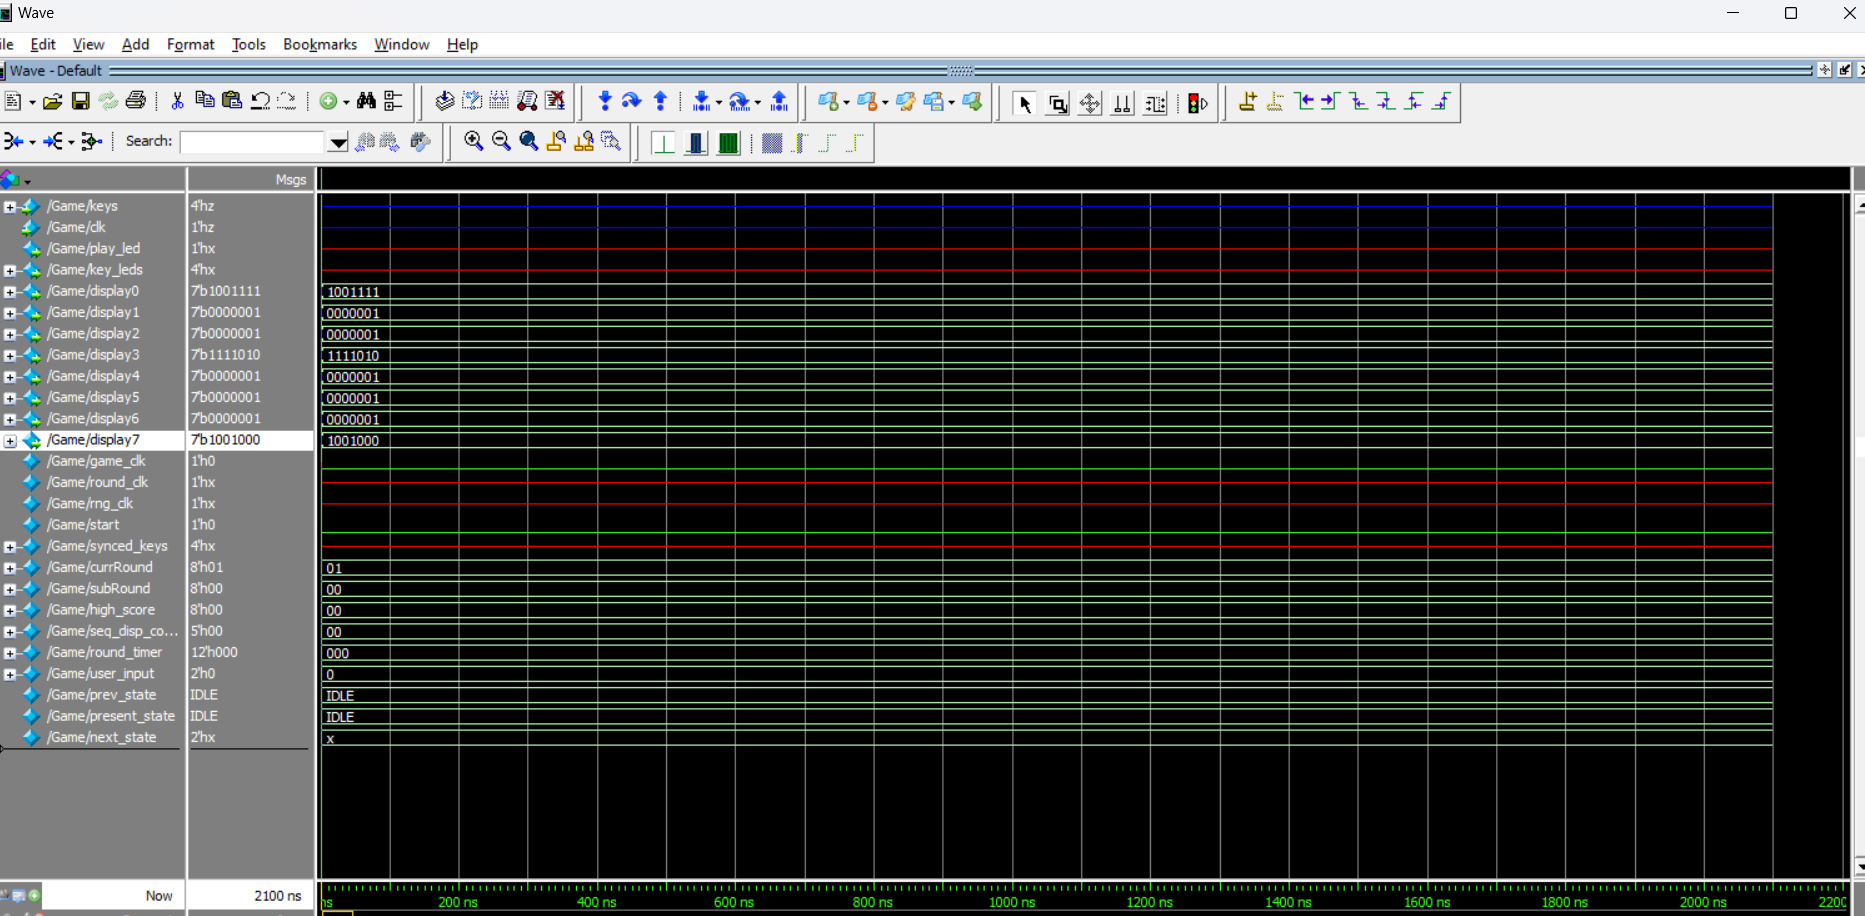
\includegraphics[width=0.75\textwidth]{images/image1.png}
    \end{center}
    \caption{Top Level Waveform}
\end{figure}

\chapter{Analysis}
The design operated successfully, meeting its primary objectives with some minor adjustments to the initial concept. The system was user-friendly and capable of supporting up to 100 rounds, though certain limitations were identified. For instance, user data could not be retained if the system was powered off, and there was no reset functionality unless the user lost the game. Despite these constraints, the game effectively randomized patterns on the board. However, the random number generator (RNG) had limited randomness due to the small number of keys used, which resulted in less variation over time. \newline \newline
From a performance perspective, the timing was sufficient for smooth gameplay, with acceptable latency and throughput to support user interactions. Space requirements were minimal, allowing the design to operate efficiently within the hardware constraints. \\\newline
For future enhancements, we aim to include an LCD screen to improve user interaction and display additional game details. We also plan to implement a more advanced RNG to produce better randomization, particularly within smaller subsets, reducing sequential patterns. Additional features such as sound integration could make the game more immersive and engaging. A potential multiplayer mode would allow one user to create a pattern while the other attempts to replicate it, fostering competition and collaboration. This feature could also have educational benefits, enhancing pattern recognition and memory skills.\\ \newline
Feedback from the poster session highlighted the importance of incorporating these features to improve user experience and broaden the design's applications. These insights will guide our future iterations of the system.


\chapter{Task Breakdown}
We collaboratively agreed on the initial concept of designing a "Simon Says" game and worked together to enhance the project by incorporating unique features to distinguish our work from other groups. Overall, our teamwork was effective, resulting in a functional and presentable final design. \newline
\textbf{Responsibilities:}
\begin{itemize}
    \item \textbf{Mari's Contributions}
    \begin{itemize}
        \item Led the system design, focusing on key functionalities such as the finite state machine (FSM), random number generator (RNG), and sequence generation. Her work ensured the core game logic was functional and scalable.
    \end{itemize}
    \item \textbf{Felix's Contributions}
    \begin{itemize}
        \item Managed the written report, prepared the presentation materials, and worked on integrating the LCD display into the design. However, when the LCD display proved unsuccessful, we adapted the design to utilize a Seven-Segment Display, ensuring the game interface was operational for the final presentation.
    \end{itemize}
\end{itemize}
Through effective collaboration and division of tasks, we were able to address challenges and present a fully functional design, showcasing our problem-solving and teamwork skills.
\chapter{Conclusion}
The "Simon Says" game project demonstrated the integration of hardware and software systems to create an engaging and interactive memory-based challenge. We delivered a functional and scalable game by designing a progressively challenging gameplay mechanism, incorporating visual and textual feedback through LEDs and a Seven-Seg Display, and ensuring high-score tracking.
Through this project, we gained hands-on experience in developing state machines, synchronizing hardware inputs, and managing persistence for user data. Additionally, we enhanced our problem-solving and debugging skills while working on real-time systems. This experience reinforced the importance of modular design and rigorous testing in achieving a reliable and user-friendly product. Overall, this project deepened our understanding of embedded systems and their potential for creating interactive applications.
\chapter{Links and References}
Project Github \url{https://github.com/azeleaButterfly/ECPE174-Final-Project}
XORshift RNG: \url{https://en.wikipedia.org/wiki/Xorshift}
\newpage

\appendix
\chapter{Other Code}
\section{Clock Divider}
\inputminted{sv}{../clockdiv.sv}
\section{Synchronizer Code}
\inputminted{sv}{../synchronizer.sv}
\section{Full Top Level Module + FSM Code}
\hypertarget{fsm_code}{Due} to the width of the text in the file, a smaller font size had to be used
\scriptsize{\inputminted{sv}{../game.sv}}

\end{document}
